\documentclass[11pt]{article}

\usepackage[margin=1in]{geometry}
\linespread{1.2}
\usepackage{amsmath,amsthm,amssymb,amsfonts}
\usepackage{hyperref}
\usepackage{enumerate}
\usepackage[noend]{algpseudocode}
%\usepackage{algorithm}
\usepackage{tikz}
\usepackage{graphicx}
\usepackage{caption,subcaption}

 
\title{Model Description}

% Replace with your name and ID below
%\author{Guoning Yu}

\date{}

\newtheorem*{thm}{Theorem}
\newtheorem*{claim}{Claim}
\newtheorem*{prop}{Proposition}
\newtheorem*{coro}{Corollary}
\newenvironment{solution}{{\par\noindent\it Solution.}}{\hfill $\square$\par}

\newcommand{\GT}{G_{tot}}
\newcommand{\VGT}{\vec{G}_{tot}}

\begin{document}

\maketitle

\section{Shape of the ``Mouse''}

%\subsection{Shoulder, spine and hip}
First of all, we introduce how the mouse is simplified for simulation purpose. As shown in figure~\ref{fig:drawing}, we take the center of mass (COM) at the middle of its hip. We assume that the direction of its movement is the direction that the COM moves. However in our description below, we use the words "forward" or "backward" with respect to the body orientation when talking about the limb movements.

For the functional parts of its body, we first define a rigid \textit{shoulder-spine-hip} frame as shown in the bottom view of figure~\ref{fig:drawing} in current stage. The ``shoulder'' and ``hip'' are of length $ l_f $ and $ l_h $, respectively, and the ``spine'' is of length $ L $. No relative movement is allowed within this structure of three parts. Moreover, the plane that this triple forms is called the \textit{horizontal plane} which is always parallel to the ground, and its normal direction is called the \textit{vertical direction}. We generally assume that the distance from the horizontal plane to the ground is fixed and defined to be the height $ H $ of the mouse. Only in some calculation related to the loads in Section~\ref{sec:load}, vertical displacement of the COM is taken into account.

\begin{figure}[h]
	\centering
	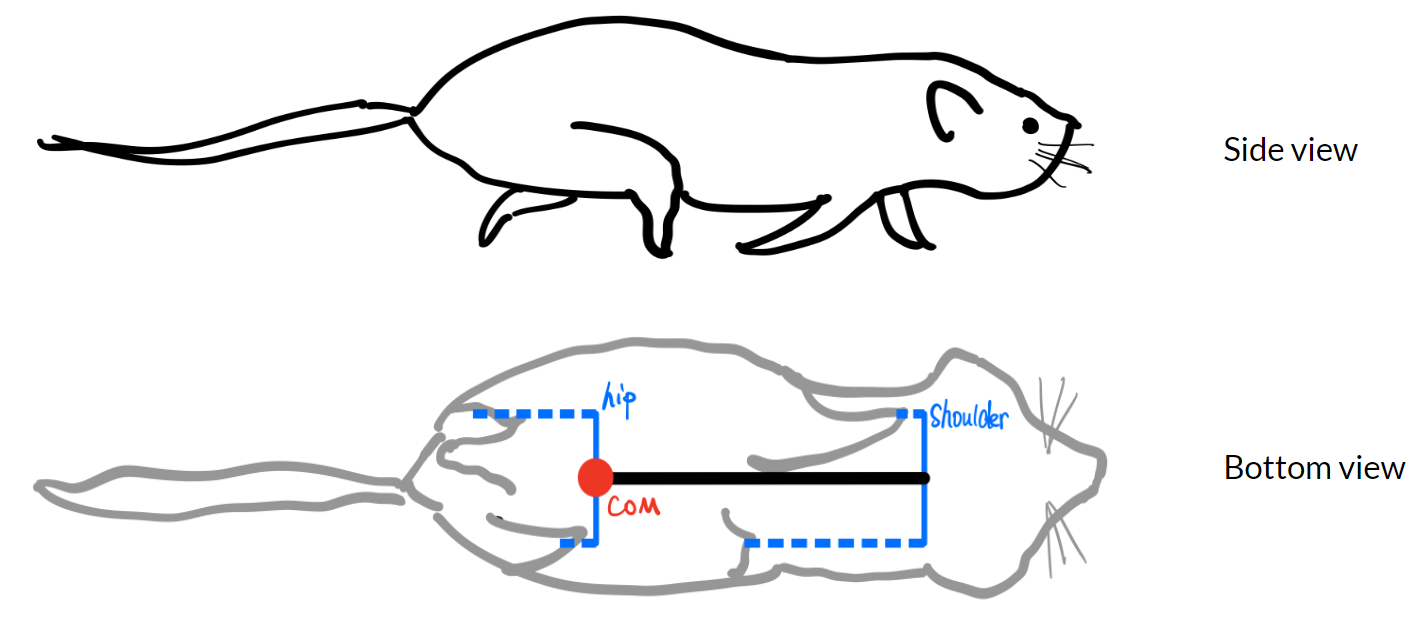
\includegraphics[width=0.6\textwidth]{side_bottom_drawing.png}
	\caption{Model simplification}
	\label{fig:drawing}
\end{figure}

The mouse is supported by its limbs, and only the paws are touching the ground. We assume that there is only one joint for each limb that connects the limb to an end of the shoulder or the hip. The only relative movements are the limb movements allowed by these four joints. When a limb is swinging, it swings forward until the paw is exactly under the joint. In other words, each joint serves as a target position in the horizontal plane for the corresponding paw if the limb is swinging. The \textit{limb length} is defined by the farthest horizontal displacement of a paw to its joint. 





\section{Forces}

Let $ m $ be the mass and $ g $ be the gravity acceleration. All external forces taken into account are the gravity force, friction force and the ground reaction force applied to each paw if it is touching the ground. We decompose the forces into horizontal and vertical directions. We indicate vectors using arrows and their magnitude without arrows.


\subsection{Horizontal forces}

\noindent\textbf{Acceleration:}

Taking a perpendicular coordinate system on the horizontal plane, let $ \vec{r}_c $ and $ \vec{v}_c=\frac{d\vec{r}_c}{dt} $ be the position and velocity vector of the COM.

\begin{figure}[h]
	\centering
	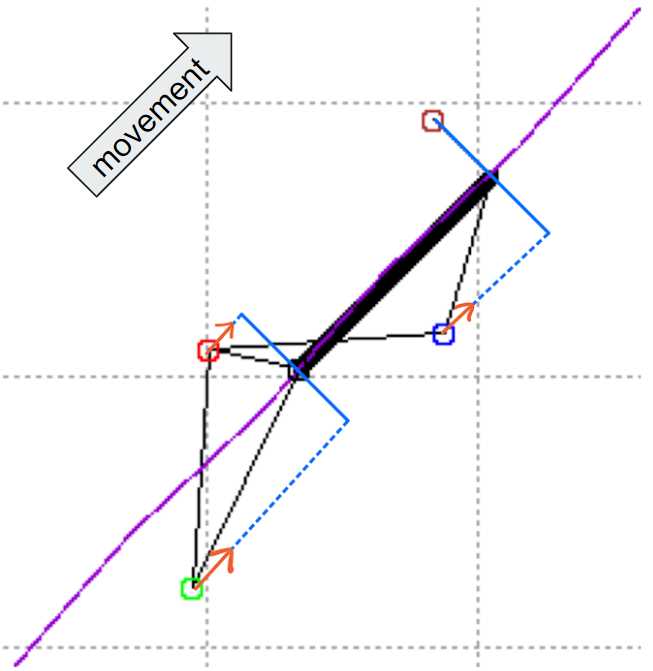
\includegraphics[width=0.4\textwidth]{horizontal_forces.png}
	\caption{Horizontal forces}
	\label{fig:horiforce}
\end{figure}

A paw touching the ground is applied a force towards its joint. Let $ \vec{F}_1, \vec{F}_2, \vec{F}_3 $ and $ \vec{F}_4 $ denote the horizontal part of ground reaction force for the front left, front right, hind left and hind right limbs, respectively. We will also refer the limbs in this order in the following context unless otherwise specified. Recall that each $ \vec{F}_i $ points to its joint, and we assume they have the same magnitude $ F_0 $.

During motion, the ground friction force can be ignored since there is only static friction. Let the air friction be $ \vec{F}_f=-\lambda \vec{v}_c $, where $ \lambda $ is the coefficient of kinetic friction of air.

\begin{figure}[h]
	\centering
	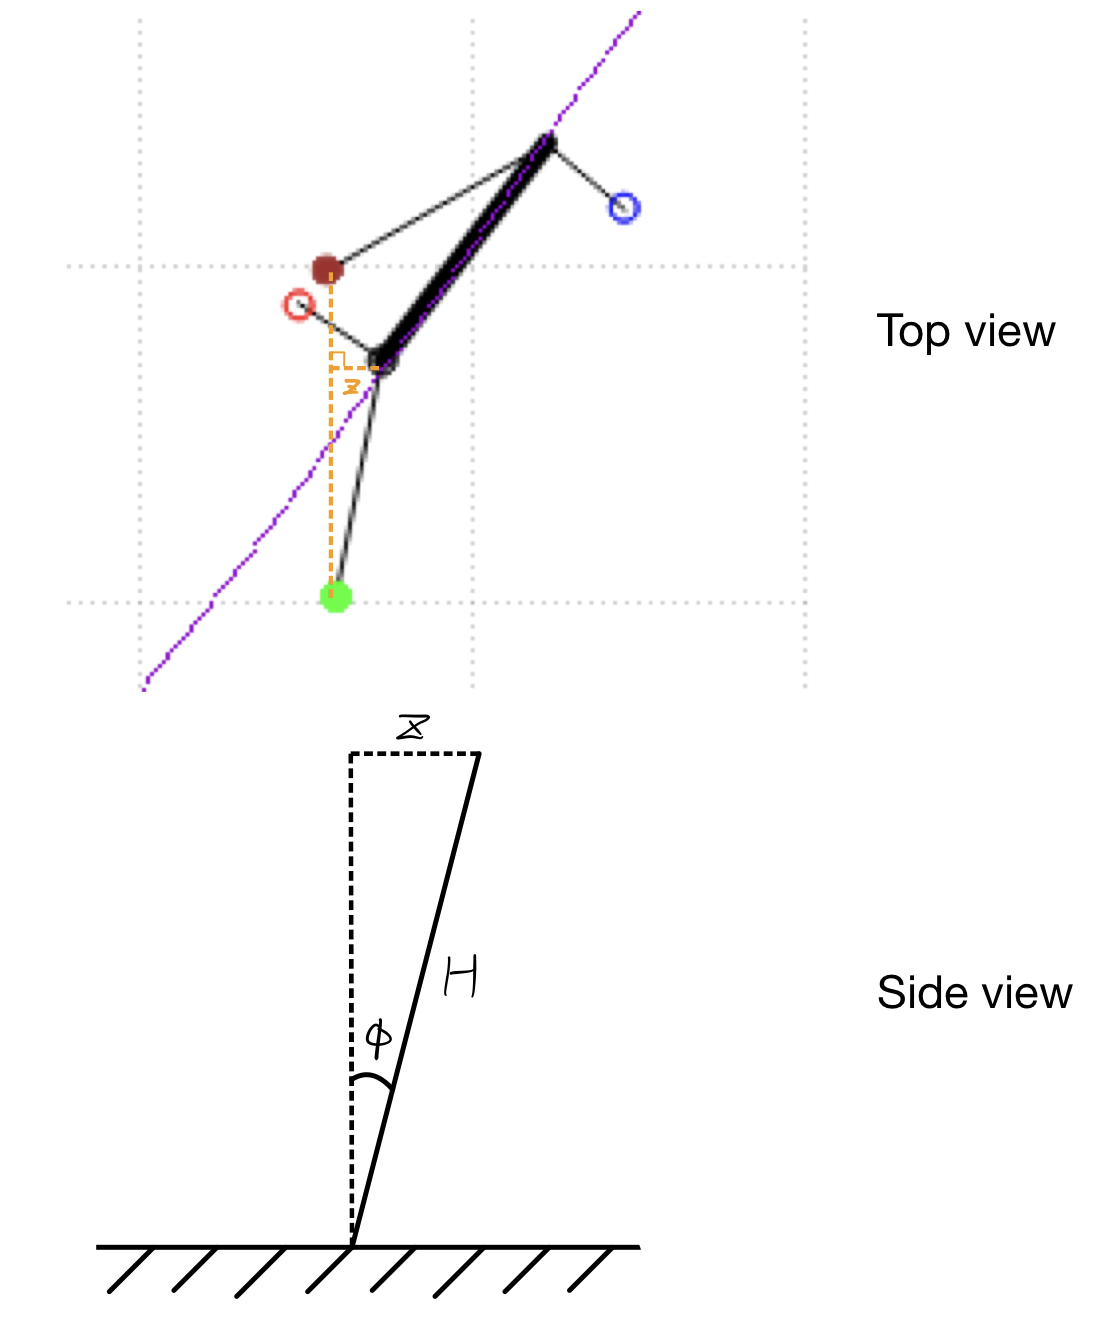
\includegraphics[width=0.5\textwidth]{inverted_pendulum}
	\caption{Horizontal forces}
	\label{fig:invtpdlm}
\end{figure}

When two limbs are supporting, as shown in figure~\ref{fig:invtpdlm}, we connect the positions of these two limbs by a \textit{supporting line segment}. Let $ \vec{z} $ be the distance vector from the supporting line segment to the COM in the horizontal plane, and let $ \phi $ be the angle of inclination. The model can be seen as a simple inverted pendulum pivoted at the supporting line segment with initial velocity $ \vec{v}_c $.  It is governed by the following equation. 
\begin{equation}
	\frac{d^2\phi}{dt^2} = \frac{g}{H} \sin\phi
\end{equation}
We take $ \phi\approx \sin\phi = \frac{z}{H} $ since $ \phi $ is small, and therefore,
\begin{equation}
	\frac{d^2 z}{dt^2} = \frac{gz}{H}
\end{equation}
This acceleration due to inertia can be taken as a \textit{inverted pendulum force} denoted by $ \vec{F}_p $ who has the direction the same as the distance vector $ \vec{z} $ and the magnitude
\begin{equation}\label{ipforce}
	F_p=m\frac{d^2 z}{dt^2}= \frac{mg}{H}\cdot z
\end{equation}
Note that Equation~\ref{ipforce} is also applicable to the case that only one limb is supporting. However, if more that two limbs are supporting, we assume that $ F_p=0 $ since the COM is always inside the supporting triangle or quadrangle.

By the Second Newton's Law, the linear velocity is governed by
\begin{equation}\label{eq:accelerationeq}
	m\frac{d \vec{v}_c}{dt} = \sum_{i=1}^4 \vec{F}_i - \lambda \vec{v}_c + \vec{F}_{p}
\end{equation}



\noindent\textbf{Rotation:} 

Since a mouse has a tail with length comparable to its body which can not be ignored, we calculate the rotation by assuming that the mouse is of length $ 2L $, and the COM is at the midpoint of the body. We take the COM as the center of rotation in the horizontal plane and consider the torques of all forces applied which create rotation. The moment of inertia of a uniform rod with negligible thickness of length $ 2L $ about the COM is
\begin{equation}
	I = \frac{mL^2}{3}
\end{equation}

By assumption, the gravity force is applied exactly at the COM, thus creates zero torque, and so as the inverted pendulum force since the it comes from the gravity force. For $ i=1,2,3$ and $ 4 $, let $ \vec{r}_i $ be the position vector of each limb in the original coordinate system. Then, the distance vector from the COM to each limb is 
\begin{equation}
	\vec{l}_i = \vec{r}_i-\vec{r}_c, i = 1,2,3,4
\end{equation}
And the torque that each ground reaction force creates is
\begin{equation}
	\vec{M}_i = \vec{l}_i \times \vec{F}_i, i = 1,2,3,4
\end{equation}

Now we calculate the air friction torque $ \vec{M}_f $.
Let $ \omega $ be the angular velocity of the body centering at the COM.
\begin{align*}
	dM_f &= s\lambda v \frac{ds}{2L}\\
	&= s\lambda s\omega \frac{ds}{2L}\\
	&= \frac{s^2\lambda \omega}{2L} ds
\end{align*}
Therefore, the torque of the friction force is 
\begin{equation}
	M_f = \int_{-L}^{L} \frac{s^2\lambda \omega}{2L} ds =  \frac{\lambda L^2}{3} \omega = \frac{\lambda I}{m} \omega 
\end{equation}



In current simulation, we assume that there is a compensation of rotating to make the gaits stable by an implementation of abductor and adductor for every limb. Let $ \psi_i $ be the angle of limb $ i $ deviate from the body orientation at its joint on the horizontal plane. The abductor and adductor tend to minimize this angle at any time, and we assume their forces are proportional to the length of extension. Let $ \vec{r}_{i,0} $ be the position vectors of each joint and $ M_A $ be the total torque of abductors and adductors from all limbs on the ground. We have
\begin{equation}
	M_A = \sum_{i=1}^{4} k_r \left(\vec{r}_{i,0} - \vec{r}_i\right) \frac{d \psi_i}{dt},
\end{equation}
where $ k_r $ is the \textit{coefficient of rotating compensation}. 

%applying biased forces to the paws in different sides. Let $ F_0 $ be the basic force applied to each paw in the horizontal direction which pushes the mouse forward. We denote the \textit{coefficient of bias} by $ \delta $ and let the actual horizontal force be
%\begin{align}
%	F_1 = F_3 = (1+\delta) F_0\\
%	F_2 = F_4 = (1-\delta) F_0
%\end{align}
%In simulation, since the direction of $ \omega $ is anticlockwise, we let $ \delta = 0.1 \omega $ for example. In this case, if the mouse is rotating anticlockwisely, the left paws would push stronger  and the right paws weaker, which compensates the rotation.

By the Second Newton's Law in angular form, we add the total torque and get
\begin{equation}
	I\frac{d\omega}{dt} = \sum_{i=1}^{4} M_i - M_f + M_A.
\end{equation}


\subsection{Vertical forces}\label{sec:load}
When talking forces not in the horizontal plane, we add another axis of coordinate along the vertical direction. In such three dimensional space, let $ \vec{G}_1, \vec{G}_2, \vec{G}_3 $ and $ \vec{G}_4 $ denote the supporting forces of the four limbs in which the order is irrelevant to the order of limbs, and assume that they are the part of ground reaction forces in the upward direction. Let $ \vec{G}_{tot} = \sum_{i=1}^{4} \vec{G}_i $ be the total supporting force, and $ \GT $ denote its magnitude. Since the mouse is not pitching in any direction, we have the torque balance equation no matter how many limbs is supporting.
\begin{equation}\label{eq:sptt}
	\sum_{i=1}^{4} \vec{l}_i \times \vec{G}_i = \vec{0}.
\end{equation}
We discuss situations of different number of limbs supporting.

\noindent\textbf{Support by $ 3 $ limbs:}
We assume that equilibrium is achieved when the COM is inside the supporting triangle. Without loss of generality, let $ G_4 = 0 $. Then, we have both equations of forces as follows.
\begin{equation}\label{eq:spt3f}
	\GT = G_1+G_2+G_3 = mg
\end{equation}
The system of Equation~\ref{eq:sptt} and \ref{eq:spt3f} has a unique solution.


\noindent\textbf{Support by $ 4 $ limbs:}
We assume that equilibrium is achieved when the COM is inside the supporting quadrangle. Similarly as above, we have the balance of forces and torques.
\begin{equation}\label{eq:spt4f}
	\GT = G_1+G_2+G_3+G_4 = mg 
\end{equation}
Note that the system of Equation~\ref{eq:sptt} and \ref{eq:spt4f} has infinite solutions. We assume that the total load is evenly distributed under the restriction~\ref{eq:sptt} and \ref{eq:spt4f}. Particularly, we minimize $ \sum_{i=1}^{4} G^2_i $ to get a unique solution. This optimization problem can be formulated and solved by linear programming.
%\begin{equation}
%	\psi = \frac{1}{2}\sum_{i=1}^{4} G^2_i
%\end{equation}


\noindent\textbf{Support by $ 2 $ limbs:}
Without loss of generality, let $ G_3 = G_4 = 0 $. Similar as the calculation of horizontal forces, we consider it as a inverted pendulum. Let $ G_{tot} $ be the the total supporting forces. By taking the centrifugal force into account, we have
\begin{equation}\label{eq:spt2f}
	\GT = G_1 + G_2 = mg\cos\phi - \frac{mv_c^2}{H}
\end{equation}
Combining Equations~\ref{eq:sptt} and \ref{eq:spt2f}, there is a unique solution for $ G_1 $ and $ G_2 $.

\noindent\textbf{Support by no more $ 1 $ limb:}
***Inverted pendulum similar as two limbs supporting.




\section{Limb Control and Simulation Results}
Now we describe the active locomotion control mechanisms by the mouse itself and present some simulation results with different set of decisions.


\subsection{Swinging a limb when unloaded or overextended}

A limb has two states during the movement: swing and stance. When it swings, both of the horizontal force and the vertical force are zero, and as pointed out previously, it moves to its joint position in the air. In the horizontal plane, let $ \vec{u}_i $ be the joint position of each limb for $ i = 1,2,3,4 $. To be more precise, the position of each paw is controlled by
\begin{equation}
	\tau_s  \frac{d \vec{r}_i}{dt} = \vec{u}_i
\end{equation}
where $ \tau_s $ is the coefficient that indicates the tendency of the paw swinging to its joint.


On the other hand, if the supporting force of a limb is not greater than $ 0 $, which means it is not supporting anymore, the paw is not supposed to be on the ground, so that the limb naturally transforms from stance to swing. Moreover, as a consequence of limited length of a limb, it can not afford to be on the ground when it is overextended. In other words, the $ i $-th limb is lifted if 
\begin{equation}\label{cond:stronglift}
	G_i<0 \quad \text{or} \quad l_i> L_i
\end{equation}

Although the lifting is necessary under condition~\ref{cond:stronglift}, by observation, a mouse would not always wait to lift a paw that is on the ground until this condition is satisfied. We assume that if the supporting force of a standing limb is very small and still decreasing, it is no longer needed to be on the ground. Therefore, we introduce a uniform threshold $ G_u\in[0,1] $ such that the $ i $-th limb is lifted if its supporting force satisfies
\begin{equation}\label{cond:weaklift}
	G_i < G_u \quad \text{and}\quad \frac{dG_i}{dt}<0.
\end{equation}

Let us call condition~\ref{cond:stronglift} the \textit{strong lifting condition} and condition~\ref{cond:weaklift} the \textit{weak lifting condition}.

\subsection{Inhibitions of swing}

For a given front (resp.~hind) limb, we call the front (resp.~hind) limb on the opposite side its \textit{contralateral} limb, and the hind (resp.~front) limb on the same side its \textit{homolateral} limb. We assume that the contralateral and homolateral limbs' swing inhibit each other as shown in figure~\ref{fig:CPG} (which will be explained further in Chapter~\ref{chap:CPG}). However, it is differently implemented under the strong and weak lifting conditions.
\begin{figure}[h]
	\centering
	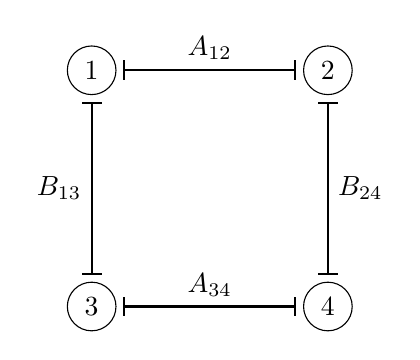
\begin{tikzpicture}
		\node[draw,circle] (x1) at (0,3) {1};
		\node[draw,circle] (x2) at (3,3) {2};
		\node[draw,circle] (x3) at (0,0) {3};
		\node[draw,circle] (x4) at (3,0) {4};
		\draw [|-|,thick] (0.4,0) to node[pos=0.5, above]{$ A_{34} $} (2.6,0);
		\draw [|-|,thick] (0.4,3) to node[pos=0.5, above]{$ A_{12} $} (2.6,3);
		\draw [|-|,thick] (0,0.4) to node[pos=0.5, left]{$ B_{13} $} (0,2.6);
		\draw [|-|,thick] (3,0.4) to node[pos=0.5, right]{$ B_{24} $} (3,2.6);
	\end{tikzpicture}
	\caption{Inhibitions of lifting}
	\label{fig:CPG}
\end{figure}

If the $ i $-th limb satisfies the strong lifting condition, it has to swing whatever state its contralateral and homolateral limbs are in. Then, the its swing inhibits both of its contralateral and homolateral limbs so that their swing terminates immediately. If the $ i $-th limb satisfies the weak lifting condition but not the strong lifting condition, it can be kept on the ground and provide both vertical and horizontal forces. In this case,  when its contralateral or homolateral limbs (or both) are swinging, it is inhibited from being lifted.



%the other limb on the same side is swinging, particularly for the hind limbs; or

\subsection{Decisions of landing a limb}

We explore two different decisions for landing a limb that is in the swing: constant swing duration and balance control.

First, it is the simplest guess that the swing of a limb is terminated some specific time $ t_{sw} $ after it begins swinging.



Second, it is nature to consider that when the mouse is losing balance, it has to put a swing limb down for supporting. Noticing that this is a global signal instead of a signal from any single limb, we assume that it decides to put down the limb that swings for the longest time (if there is one). We define the signal of losing balance by that the total supporting force is fast decreasing, so that another threshold $ k_v\in(0,\infty) $ is introduced. The mouse is losing balance when
\begin{equation}
	-\frac{d\GT}{dt}>k_v.
\end{equation}



\section{CPG Model Implementation}\label{chap:CPG}
%For $ i = 1,2,3,4 $, let $ \theta_i $ be the phase of oscillators of each limb CPG. It is described by 



\section{Simulation Results}\label{chap:simulation}

In the simulation, we let $ G_{tot} = 0 $ when more than two limbs is standing, and $ G_{tot} = 1 $ when only one limb is standing.



\newpage

\begin{tabular}{|c|l|}
	\hline
	\multicolumn{1}{|c|}{Parameters} & \multicolumn{1}{|c|}{Meaning} \\
	\hline
	&  \\
	\hline
	&  \\
	\hline
	&  \\
	\hline
	&  \\
	\hline
	&  \\
	\hline
	&  \\
	\hline
	&  \\
	\hline
	&  \\
	\hline
\end{tabular}


\bibliographystyle{plain}
\bibliography{Mouse_Locomotion.bib}


\end{document}
